\documentclass[12pt]{article}
\usepackage{geometry}
\geometry{left=2.5cm,right=2.5cm,top=2.5cm,bottom=2.5cm}

\usepackage{comment}
% \usepackage{indentfirst} 
\usepackage{booktabs}
\usepackage{enumerate}
\usepackage{physics}
\usepackage{graphicx}
\usepackage{setspace}
\setlength{\parindent}{0pt}
\setstretch{1.2} 
\usepackage{diagbox}
\usepackage{amsmath,amsfonts,graphicx,amssymb,bm,amsthm}
\allowdisplaybreaks
\usepackage{algorithm,algorithmicx}
\usepackage[noend]{algpseudocode}
\usepackage{fancyhdr}
\usepackage{tikz}
\usepackage{dot2texi}
\usepackage{tikz}
\usetikzlibrary{shapes,arrows}
\usetikzlibrary{arrows,automata}
\usepackage{hyperref}
\setlength{\headheight}{14pt}

\date{\today}

\usepackage{fancyhdr}
\pagestyle{fancy}
\lhead{QCQI Exercises}         
\chead{}          
\rhead{}           

\lfoot{}          
\cfoot{\thepage}  
\rfoot{}          
 
 

 
 
 
\title{\textbf{QCQI Exercises}}

\author{Huiping Lin}
 
 
 
\begin{document}
 \bibliographystyle{plain}
\maketitle
%\tableofcontents

\section*{Chapter 2}

\subsection*{Exercise 2.1}
\begin{align}
\left(\begin{array}{c}
1 \\
-1
\end{array}\right)+\left(\begin{array}{l}
1 \\
2
\end{array}\right)-\left(\begin{array}{l}
2 \\
1
\end{array}\right)=0.
\end{align}

\subsection*{Exercise 2.2}
\begin{align}
    A=\begin{pmatrix}0&1\\1&0\end{pmatrix}.
\end{align}

\subsection*{Exercise 2.3}

For each $v_i$, we have $A\ket{v_i}=\sum_j A_{ji}\ket{w_j}$. For each $w_j$, we have  $B\ket{w_j}=\sum_k B_{kj}\ket{x_k}$.

So for each $v_i$, we have:
\begin{align}
     (BA)\ket{v_i}&=B(A\ket{v_i}=B(\sum_j A_{ji}\ket{w_j})=\sum_j A_{ji}B\ket{w_j}\\
     &=\sum_j A_{ji}\sum_k B_{kj}\ket{x_k}=\sum_{jk} B_{kj} A_{ji}\ket{x_k}=\sum_k (BA)_{ki}\ket{x_k}.
\end{align}

Therefore the matrix presentation for linear transformation $BA$ is the matrix product of the matrix representation for $B$ and $A$.

\subsection*{Exercise 2.4}
 If $I$ is the identity operator, then for each $\ket{v_i}$, there must be $I\ket{v_i}=\sum_j I_{ji}v_i=v_i$. So $I_{ji}=\delta_{ji}$, which means the matrix representation of $I$ is the identity matrix.
 
 \subsection*{Exercise 2.5}
 
 If $(\ket{u},\ket{v})=\sum_i u_i^*v_i$, then we can verify that:
 \begin{enumerate}
     \item For $\ket{v}$ and $\sum_i \lambda_i\ket{w_i}$, we have:
     \begin{align}
              (\ket{v},\sum_i \lambda_i\ket{w_i})=\sum_j v_j^*\sum_i \lambda_i w_{ij}= \sum_i\lambda_i(\sum_j v_j^* w_{ij})=\sum_i\lambda_i(\ket{v},\ket{w_i}).
         \end{align}
     \item For $\ket{v}$ and $\ket{w}$, we have:
     \begin{align}
          (\ket{v},\ket{w})=\sum_i v_i^*w_i=\sum_i w_iv_i^*=\sum_i(w_i^*v_i)^*=(\sum_iw_i^*v_i)^*=(\ket{w},\ket{v})^*.
     \end{align}
     \item For $\ket{v}$, we have:
     \begin{align}
              (\ket{v},\ket{v})=\sum_i v_i^*v_i=\sum_i|v_i|^2\geq0.
         \end{align}
     The equivalence holds only when all $v_i=0$, which means $\ket{v}=0$.
 \end{enumerate}
 
\subsection*{Exercise 2.6}
We can verify that:
\begin{align}
\left(\sum_i \lambda_i\ket{w_i},\ket{v}\right)  =\left(\ket{v},\sum_i \lambda_i\ket{w_i}\right)^*  =\left(\sum_i\lambda_i(\ket{v},\ket{w_i})\right)^*=\sum_i\lambda_i^*(\ket{w_i},\ket{v}).
         \end{align}

\subsection*{Exercise 2.8}
Use the induction method. 

First, $v_1$ is normal, and the set $\{v_1\}$ is orthonormal.

Now suppose the vectors $v_1,v_2,\cdots,v_{j-1}$ are orthonormal, which means $\langle v_m|v_n\rangle =\delta_{mn}$ for all $m,n\leq j-1$.

For any $\ket{v_i}$ and $\ket{v_j}$ with $j>i$, we have: 
\begin{align}
         \langle v_i|v_j\rangle&=\frac{1}{|w_j'|}\left(\langle v_i|\left(|w_j\rangle -\sum_{t=1}^{j-1}\langle v_t|w_j\rangle\ket{v_t}\right)\right)\\
         &=\frac{1}{|w_j'|}\left(\langle v_i|w_j\rangle -\sum_{i=1}^{j-1}\langle v_t|w_j\rangle\langle v_i|v_t\rangle\right)\\
         &=\frac{1}{|w_j'|}\left(\langle v_i|w_j\rangle -\sum_{i=1}^{j-1}\langle v_t|w_j\rangle\delta_{it}\right)\\
         &=\frac{1}{|w_j'|}\left(\langle v_i|w_j\rangle -\langle v_i|w_j\rangle\right)=0.
         \end{align}
Therefore $\ket{v_j}$ is orthogonal to all $\ket{v_i}$ for $i<j$. Additionally $\ket{v_j}$ is normal.

So the Gram-Schmidt procedure produces an orthonormal basis.

\subsection*{Exercise 2.9}
\begin{align}
X=\begin{pmatrix}0&1\\1&0\end{pmatrix}=|1\rangle\langle 0|+|0\rangle\langle 1|.
\end{align}
\begin{align}
Z=\begin{pmatrix}1&0\\0&-1\end{pmatrix}=|0\rangle\langle 0|-|1\rangle\langle 1|.
         \end{align}
     \begin{align}
Y=\begin{pmatrix}0&-i\\i&0\end{pmatrix}=-i|1\rangle\langle 0|+i|0\rangle\langle 1|.
         \end{align}
     
\subsection*{Exercise 2.10}
$M=\ket{v_j}\bra{v_k}$, and its each element is: $M_{ab}=\bra{v_a}M\ket{v_b}=\delta_{aj}\delta_{bk}$. So only $M_{jk}=1$, and other elements are all $0$.

\subsection*{Exercise 2.11}
$X$ has eigenvalue $1$ and eigenvector $1/\sqrt 2(\ket{0}+\ket{1})$, eigenvalue $-1$ and eigenvector $1/\sqrt 2(\ket{0}-\ket{1})$.

$Y$ has eigenvalue $1$ and eigenvector $1/\sqrt 2(\ket{0}+i\ket{1})$, eigenvalue $-1$ and eigenvector $1/\sqrt 2(\ket{0}-i\ket{1})$.

$Z$ has eigenvalue $1$ and eigenvector $\ket{0}$, eigenvalue $-1$ and eigenvector $\ket{1}$.

So the diagonal representations are:
\begin{align}
X=\frac{1}{2}(\ket{0}+\ket{1})(\bra{0}+\bra{1})-\frac{1}{2}(\ket{0}-\ket{1})(\bra{0}-\bra{1}).
 \end{align}
\begin{align}
Y=\frac{1}{2}(\ket{0}+i\ket{1})(\bra{0}-i\bra{1})-\frac{1}{2}(\ket{0}-i\ket{1})(\bra{0}+i\bra{1}).
 \end{align}
\begin{align}
Z=\ket{0}\bra{0}-\ket{1}\bra{1}.
 \end{align}

\subsection*{Exercise 2.12}

${\rm det}(A-\lambda I)=(1-\lambda)^2 = 0$ has only one eigenvalue $\lambda = 1$, but ${\rm rank}(I-A)<2$. So it is not diagonalizable.

\subsection*{Exercise 2.13}

For any two vectors $\ket{a},\ket{b}$, we have:
\begin{align}
(\ket{a},(\ket{w}\bra{v})^\dagger\ket{b})&=((\ket{w}\bra{v})\ket{a},\ket{b})\\
&=(\bra{v}\ket{a}\ket{w},\ket{b})\\
&=\bra{v}\ket{a}^*\bra{w}\ket{b}\\
&=\bra{a}\ket{v}\bra{w}\ket{b}\\
&=(\ket{a},(\ket{v}\bra{w})\ket{b}).
 \end{align}

So $(\ket{w}\bra{v})^\dagger=\ket{v}\bra{w}$.

\subsection*{Exercise 2.14}
Because
\begin{align}
\left(\left(\sum_{i} a_{i} A_{i}\right)^{\dagger}|v\rangle,|w\rangle\right) &=\left(|v\rangle, \sum_{i} a_{i} A_{i}|w\rangle\right) \\
&=\sum_{i} a_{i}\left(A_{i}^{\dagger}|v\rangle,|w\rangle\right) \\
&=\left(\sum_{i} a_{i}^{*} A_{i}^{\dagger}|v\rangle,|w\rangle\right),
 \end{align}
So the equation holds, which means the adjoint operation is anti-linear.

\subsection*{Exercise 2.15}
Because
\begin{align}
\left((A^\dagger)^\dagger\ket{v},|w\rangle\right)
&=(\ket{v},A^\dagger \ket{w}) \\
&=(A^\dagger\ket{w},\ket{v})^*\\
&=(\ket{w},A\ket{v})^*\\
&=(A\ket{v},\ket{w}),
 \end{align}
so $(A^\dagger)^\dagger = A$.

\subsection*{Exercise 2.16}
\begin{align}
P^2&=\left(\sum_{i=1}^{k}\ket{i}\bra{i}\right)\left(\sum_{i=1}^{k}\ket{i}\bra{i}\right)\\
&=\sum_{i,j=1}^k \ket{i}\bra{i}\ket{j}\bra{j}=\sum_{i,j=1}^k \bra{i}\ket{j}\ket{i}\bra{j}\\
&=\sum_{i,j=1}^k\delta_{ij}\ket{i}\bra{j}\\
&=\sum_{i=1}^k\ket{i}\bra{i}=P.
 \end{align}

\subsection*{Exercise 2.17}
We know that any normal matrix $A$ can be diagonalized by an unitary matrix $U$, which means $A=U^\dagger DU$, where $D$ is a diagonal matrix.

If $A$ is Hermitian, then for any eigenvalue $i$ and the corresponding eigenvector $\ket{i}$ for $A$, we have $A\ket{i}=i\ket{i}$, and $A^{\dagger}\ket{i} = i^* \ket{i}$. Additionally, $A=A^\dagger$, so $A\ket{i}=A^\dagger \ket{i}$, which means $i\ket{i}=i^*\ket{i}$. So $i=i^*$, which means all eigenvalues of $A$ are real.

If all eigenvalues of $A$ are real, which means $D=D^\dagger$, then $U^\dagger DU=(U^\dagger DU)^\dagger = U^\dagger D^\dagger U$, so $A=A^\dagger$, which means $A$ is Hermitian. 

\subsection*{Exercise 2.18}
 Because for any unitary matrix $U$, we have $U^\dagger U = I$. And for any eigenvalue $i$ and the corresponding eigenvector $\ket{i}$, we have $U\ket{i}=i\ket{i}$. Additionally, $\bra{i}U^\dagger U\ket{i}=\bra{i}i^* i\ket{i}=|i|^2\bra{i}\ket{i}$, while we also have $\bra{i}U^\dagger U\ket{i}=\bra{i}\ket{i}$. So $|i| = 1$.

\subsection*{Exercise 2.20}

For $A'$, we have:
\begin{align}
A_{i j}' &= \bra{v_i}A\ket{v_j}\\
&=\sum_{k,t}\bra{v_i}\ket{w_k}\bra{w_k}A\ket{w_t}\bra{w_t}\ket{v_j}\\
&=\sum_{k,t}\bra{v_i}\ket{w_k}A_{kl}''\bra{w_t}\ket{v_j}
\end{align}

\subsection*{Exercise 2.21}
If $M$ is Hermitian, then $M=M^\dagger$, with $M=(P+Q)M(P+Q)=PMP+PMQ+QMP+QMQ$, where $P$ is the projector onto the $\lambda$ eigenspace, and $Q$ is the projector onto the orthogonal complement space. So $PMQ$ and $QMP$ are both $0$, and $M=PMP+QMQ$. We now prove $QMQ$ is normal. Because we have:
\begin{align}
QMQQM^\dagger Q = QM^\dagger QQMQ,
\end{align}
so $QMQ$ is normal. Here we use $M=M^\dagger$ to simplify the proof. By the induction, $QMQ$ is diagonal with respect to some orthonormal basis for $Q$, and $PMP$ is already diagonal with respect to some orthonormal basis for $P$.

\subsection*{Exercise 2.22}

If $H\ket{a}=a\ket{a}$, $H\ket{b}=b\ket{b}$, where $a,b$ are two differnet eigenvalues, then we have:
\begin{align}
\bra{b}H\ket{a}=\bra{b}a\ket{a}=a\bra{b}\ket{a}\\
=\bra{a}H\ket{b}=\bra{a}b\ket{b}=b\bra{b}\ket{a}.
\end{align}

Because $a\neq b$, so we must have $\bra{b}\ket{a}=0$, which means $\ket{a}$ and $\ket{a}$ are orthogonal.

\subsection*{Exercise 2.23}
Because for any projector $P$, we have $P^2=P$. Then for any eigenvalue $i$ and the corresponding eigenvector $\ket{i}$, we have $P^2\ket{i}=P(P\ket{i})=P(i\ket{i})=i(P\ket{i})=i^2\ket{i}$, so $i^2\ket{i}=i\ket{i}$. So $i^2 = i$, which means $i=0$ or $i=1$.

\subsection*{Exercise 2.24}

For any positive operator, we can write it as: 
\begin{align}
A&=\frac{1}{2}(A+A^\dagger)+i\frac{1}{2i}(A-A^\dagger)\\
&=B+iC.
\end{align}

It's evident that $B=1/2(A+A^\dagger)$ and $C=1/2i(A-A^\dagger)$ are both Hermitian. Then for any vector $\ket{v}$, we have:
\begin{align}
\bra{v}A\ket{v}=\bra{v}(B+iC)\ket{v}=\bra{v}B\ket{v}+i\bra{v}C\ket{v}.
\end{align}

Because $B$ and $C$ are both Hermitian, so $\bra{v}B\ket{v}$ and $\bra{v}C\ket{v}$ are both real number. And $A$ is a positive operator, so we should have $\bra{v}A\ket{v}$ be real, so $\bra{v}C\ket{v}=0$. Therefore we have $A=A^\dagger$, which means $A$ is Hermitian.

\subsection*{Exercise 2.25}
For any operator $A$ and vector $\ket{v}$, we have:
\begin{align}
    \bra{v}A^\dagger A\ket{v}=|A\ket{v}|^2\geq 0.
\end{align}

So $A^\dagger A$ is positive.


\subsection*{Exercise 2.28}
\begin{align}
(A\otimes B)^*=\begin{pmatrix}
A_{11}^* B^*&A_{12}^*B^* & \cdots & A_{1n}^*B^*\\
A_{21}^* B^*&A_{22}^*B^* & \cdots & A_{2n}^*B^*\\
\vdots & \vdots & \vdots &\vdots \\
A_{n1}^* B^*&A_{n2}^*B^* & \cdots & A_{nn}^*B^*
\end{pmatrix}=A^*\otimes B^*
\end{align}
\begin{align}
(A\otimes B)^T=\begin{pmatrix}
A_{11} B^T&A_{21}B^T & \cdots & A_{n1}B^T\\
A_{12} B^T&A_{22}B^T & \cdots & A_{n2}B^T\\
\vdots & \vdots & \vdots &\vdots \\
A_{1n} B^T&A_{2n}B^T & \cdots & A_{nn}B^T
\end{pmatrix}=A^*\otimes B^*
\end{align}
\begin{align}
(A\otimes B)^\dagger=\begin{pmatrix}
A_{11}^* B^\dagger&A_{21}^* B^\dagger & \cdots & A_{n1}^*  B^\dagger\\
A_{12}^* B^\dagger&A_{22}^*B^\dagger & \cdots & A_{n2}^*B^\dagger\\
\vdots & \vdots & \vdots &\vdots \\
A_{1n}^* B^\dagger&A_{2n}^*B^\dagger & \cdots & A_{nn}^*B^\dagger
\end{pmatrix}= A^\dagger \otimes B^\dagger
\end{align}

\subsection*{Exercise 2.29}

For any two unitary operator $U_1$ and $U_2$, we have:
\begin{align}
(U_1\otimes U_2)^\dagger (U_1\otimes U_2) &=(U_1^\dagger\otimes U_2^\dagger) (U_1\otimes U_2)\\
&=(U_1^\dagger U_1)\otimes (U_2^\dagger U_2)=I\otimes I=I.
\end{align}

\subsection*{Exercise 2.30}

For any two Hermitian operator $H_1$ and $H_2$, we have:
\begin{align}
(H_1\otimes H_2)^\dagger (H_1\otimes H_2) &=(U_1^\dagger\otimes U_2^\dagger) (U_1\otimes U_2)\\
&=(U_1^\dagger U_1)\otimes (U_2^\dagger U_2)=I\otimes I=I.
\end{align}

\subsection*{Exercise 2.31}

For any two positive operator $A_1$ and $A_2$, we have:
\begin{align}
\bra{u}\otimes\bra{v}(A_1\otimes A_2)\ket{v}\otimes\ket{u}=
\bra{u}A\ket{u}\bra{v}B\ket{v}\geq 0.
\end{align}

\subsection*{Exercise 2.32}

For any two projectors $P_1$ and $P_2$, we have:
\begin{align}
(P_1\otimes P_2)^2=P_1^2 \otimes P_2^2 = P_1\otimes P_2.
\end{align}


\subsection*{Exercise 2.33}

Because we can write the Hadmard operator of one qubit as:

\begin{align}
H &=\frac{1}{\sqrt{2}}[(|0\rangle+|1\rangle)\langle 0|+(|0\rangle-|1\rangle)\langle 1|]\\
&=\frac{1}{\sqrt{2}}[|0\rangle\langle 0|+| 1\rangle\langle 0|+| 0\rangle\langle 1|-| 1\rangle\langle 1|] \\
&=\frac{1}{\sqrt{2}} \sum_{x, y\in\{0,1\}}(-1)^{x \cdot y}|x\rangle\langle y|
\end{align}

So for $n$ qubits, we have:
\begin{align}
H^{\otimes n} &=\frac{1}{\sqrt{2^{n}}} \sum_{x_1, y _1\in\{0,1\}}(-1)^{x_{1} \cdot y_{1}}\left|x_{1}\right\rangle\langle y_{1}|\otimes \sum_{x_{2}, y_{2}\in\{0,1\}}(-1)^{x_{2} \cdot y_{2}}| x_{2}\rangle\left\langle y_{2}\right| \otimes \cdots \\
&=\frac{1}{\sqrt{2^{n}}} \sum_{x, y\in\{0,1\}^n}(-1)^{x \cdot y}|x\rangle\langle y|.
\end{align}

And we can calculate $H^{\otimes 2}$:

\begin{align}
H^{\otimes 2}=~& \frac{1}{2}[|00\rangle\langle 00|+| 01\rangle\langle 00|+| 00\rangle\langle 01|-| 01\rangle\langle 01|\\
&+|10\rangle\langle 00|+| 11\rangle\langle 00|+| 10\rangle\langle 01|-| 11\rangle\langle 01| \\
&+|00\rangle\langle 10|+| 01\rangle\langle 10|+| 00\rangle\langle 11|-| 01\rangle\langle 11| \\
&-|10\rangle\langle 10|-| 11\rangle\langle 10|-| 10\rangle\langle 11|+| 11\rangle\langle 11|] \\
=&\begin{pmatrix}
1 & 1 & 1 & 1 \\
1 & -1 & 1 & -1 \\
1 & 1 & -1 & -1 \\
1 & -1 & -1 & 1
\end{pmatrix}
\end{align}

\subsection*{Exercise 2.34}
Let 
\begin{align}
A=\begin{pmatrix}3 &4\\4 &3\end{pmatrix}.
\end{align}

Then ${\rm det}(A-\lambda I)=(4-\lambda)^2-9$. Therefore $A$ has two eigenvalues: $\lambda_1=1$ and $\lambda_2 = 7$. The eigenvectors are $\ket{\alpha}=1/\sqrt 2(\ket{0}-\ket{1})$ and $\ket{\beta}=1/\sqrt 2(\ket{0}+\ket{1})$ respectively.

Therefore, we can rewrite $A$ as:

\begin{align}
A=\begin{pmatrix}3 &4\\4 &3\end{pmatrix}=\ket{\alpha}\bra{\alpha}+7\ket{\beta}\bra{\beta}.
\end{align}

So its root is:
\begin{align}
\sqrt A&=\begin{pmatrix}3 &4\\4 &3\end{pmatrix}=\ket{\alpha}\bra{\alpha}+\sqrt 7\ket{\beta}\bra{\beta}\\
&=\frac{1}{2}\begin{pmatrix}1+\sqrt 7 &-1+\sqrt 7\\-1+\sqrt 7 &1+\sqrt 7\end{pmatrix}.
\end{align}

Its logarithm is:
\begin{align}
\sqrt A&=\begin{pmatrix}3 &4\\4 &3\end{pmatrix}=\log 1 \ket{\alpha}\bra{\alpha}+\log 7\ket{\beta}\bra{\beta}\\
&=\frac{\log 7}{2}\begin{pmatrix}1&1\\1&1\end{pmatrix}.
\end{align}

\subsection*{Exercise 2.35}

Let $\vec v = (v_1,v_2,v_3)$, then we have:
\begin{align}
\vec v\cdot \vec \sigma&=\sum_{i=1}^3 v_i\cdot\sigma_i\\
&=\begin{pmatrix} v_3 & v_1-iv_2 \\ v_1+iv_2 & -v_3\end{pmatrix}.
\end{align}

Additionally,
\begin{align}
{\rm det}(\vec v\cdot \vec \sigma-\lambda I)=\lambda^2-(v_1^2+v_2^2+v_3^2)=\lambda^2-1.
\end{align}

Therefore, the eigenvalues are $\lambda_1=1$, and $\lambda_2=-1$. Assume the eigenvectors are $\ket{\lambda_1}$ and $\ket{\lambda_2}$. So we can write $\vec v\cdot \vec \sigma$ as:
\begin{align}
\vec v\cdot \vec \sigma=\ket{\lambda_1}\bra{\lambda_1}-\ket{\lambda_2}\bra{\lambda_2}.
\end{align}

Therefore, 
\begin{align}
\exp(i\theta \vec v\cdot \vec \sigma)=\exp(i\theta)\ket{\lambda_1}\bra{\lambda_1}+\exp(-i\theta)\ket{\lambda_2}\bra{\lambda_2}.
\end{align}

\subsection*{Exercise 2.37}
\begin{align}
{\rm tr}(AB)=\sum_i(AB)_{ii}=\sum_{i,j}A_{ij}B_{ji}=\sum_{ji}B_{ji}A_{ij}=\sum_j(AB)_{jj}={\rm tr}(BA).
\end{align}

\subsection*{Exercise 2.38}
\begin{align}
{\rm tr}(A+B)&=\sum_i(A_{ii}+B_{ii})=\sum_i A_ii + \sum_i B_ii = {\rm tr}(A)+{\rm tr}(B).
\end{align}
\begin{align}
{\rm tr}(zA)&=\sum_izA_{ii}=z\sum_i A_{ii}=z {\rm tr}(A).
\end{align}

\subsection*{Exercise 2.39}

\begin{enumerate}[(1)]
\item We now prove this definition satisfies the 3 rules of inner product.
\begin{align}
(A,A)={\rm tr}(A^\dagger A)=\sum_{ij}|A_{ij}|^2\geq 0.
\end{align}
The equation holds only when $A = 0$.

\begin{align}
(A,B)^*=({\rm tr}(A^\dagger B))^*={\rm tr}((A^\dagger B)^\dagger)={\rm tr}(B^\dagger A)=(B,A).
\end{align}
\begin{align}
(A,\sum_i \lambda_i B_i)&={\rm tr}\left(A^\dagger \left(\sum_i \lambda_i B_i\right)\right)={\rm tr}\left(\sum_i \lambda_i A^\dagger B_i\right)\\
&=\sum_i \lambda_i{\rm tr}\left( A^\dagger B_i\right)=\sum_i \lambda_i(A,B_i).
\end{align}

\item 
Any linear transformation from $V$ to $V$ can be represented as a $d \times d$ matrix, where $V$ is a $d-$dimensional space.

Because the number of independent $d\times d$ matrix is $d^2$, so $L_v$ has dimension $d^2$.

\item Let the orthonormal basis of $V$ be $\ket{v_1},\ket{v_2},\cdots,\ket{v_d}$. Then define 3 sets of Hermitian matrices: $A_{ij} = 1/2(\ket{v_i}\bra{v_j}+\ket{v_j}\bra{v_i})$, where $1\leq i<j\leq d$, and
$B_{ij}=1/2(\ket{v_i}\bra{v_j}-\ket{v_j}\bra{v_i})$, where $1\leq i<j\leq d$, and $C_i=\ket{v_i}\bra{v_i}$, where $1\leq i\leq d$. The set $\{A_{ij},B_{ij},C_i\}$ is an orthonormal basis for $L_v$.

\end{enumerate} 

\subsection*{Exercise 2.43}
\begin{align}
\sigma_j\sigma_k=\frac{[\sigma_j,\sigma_k]+\{\sigma_j,\sigma_k\}}{2}.
\label{2.43}
\end{align}

When $j\neq k$, $\{\sigma_j,\sigma_k\}=0$, and when $j=k$. $\sigma_j\sigma_k=I$. So $\{\sigma_j,\sigma_k\}=2\delta_{jk}I$. Additionally, $[\sigma_j,\sigma_k]=2i\sum_{l=1}^{3}\epsilon_{jkl}\sigma_l$.

Therefore, using equation \ref{2.43}, we have:
\begin{align}
\sigma_j\sigma_k=\delta_{jk}I+i\sum_{l=1}^{3}\epsilon_{jkl}\sigma_l.
\end{align}

\subsection*{Exercise 2.44}

If $[A,B]=0$ and $\{A,B\}=0$, then $AB+BA=AB-BA= 0$. So $BA = 0$.

Because $A$ is invertible, then $BAA^{-1}=BI=0$. So $B$ must be $0$. 

\subsection*{Exercise 2.45}
\begin{align}
\left[A,B\right]^\dagger  =(AB-BA)^\dagger=(AB)^\dagger-(BA)^\dagger = B^\dagger A^\dagger-A^\dagger B^\dagger = \left[B^\dagger ,A^\dagger \right]
\end{align}

\subsection*{Exercise 2.47}
Because $A,B$ are Hermitian, so $A=A^\dagger$ and $B=B^\dagger$. Use the conclusion of 2.45 and 2.46, we have:
\begin{align}
(i[A,B])^\dagger=-i[B^\dagger,A^\dagger]=-i[B,A]=i[A,B].
\end{align}

So $i[A,B]$ is Hermitian.

\subsection*{Exercise 2.48}
\begin{enumerate}[(1)]
    \item For a positive matrix $P$, we have $P=\sum_i\lambda_i\ket{i}\bra{i}$, where $\lambda_i\geq 0$.
    
    So $J=\sqrt{P^\dagger P}=\sum_i\sqrt{\lambda_i^2}\ket{i}\bra{i}=P$. Therefore the polar decomposition is $P=IP$.
    
    \item For a unitary matrix $U$, we have $U^\dagger U = I$, so $J=\sqrt{U^\dagger U}=I$. Therefore the polar decomposition is $U=UI$.
    
    \item For a Hermitian matrix $H$, we have $H=\sum_i\lambda_i\ket{i}\bra{i}$, where $\lambda_i$ are all real.
    
     So $J=\sqrt{H^\dagger H}=\sum_i\sqrt{\lambda_i^2}\ket{i}\bra{i}=\sum_i|\lambda_i|\ket{i}\bra{i}$. Therefore the polar decomposition is $H=U\sum_i|\lambda_i|\ket{i}\bra{i}$, where $U=\sum_i\ket{e_i}\bra{i}$.
\end{enumerate}

\subsection*{Exercise 2.49}

For a normal matrix $A$, we have $A=\sum_i\lambda_i\ket{i}\bra{i}$. So $J=\sqrt{A^\dagger A}=\sum_i\sqrt{\lambda_i^*\lambda}\ket{i}\bra{i}=\sum_i|\lambda_i|\ket{i}\bra{i}$. Therefore the polar decomposition is $A=U\sum_i|\lambda_i|\ket{i}\bra{i}$, where $U=\sum_i\ket{e_i}\bra{i}$.

\subsection*{Exercise 2.50}

\begin{align}
A=\begin{pmatrix}1&0\\1&1\end{pmatrix},A^\dagger A=\begin{pmatrix}2&1\\1&1\end{pmatrix}.
\end{align}

We have ${\rm det}(A^\dagger A-\lambda I)=(2-\lambda)(1-\lambda)-1=\lambda^2-3\lambda+1$.

So the eigenvalues are $\lambda_1=(3+\sqrt{5})/2$ and $\lambda_2=(3-\sqrt{5})/2$, with the eigenvectors:
\begin{align}
\ket{v_1}=\frac{1}{\sqrt{10-2\sqrt 5}}\begin{pmatrix}2\\-1+\sqrt 5\end{pmatrix},
\ket{v_2}=\frac{1}{\sqrt{10+2\sqrt 5}}\begin{pmatrix}2\\-1-\sqrt 5\end{pmatrix}.
\end{align}

So $J=\sqrt{A^\dagger A}=\sqrt{\lambda_1}\ket{v_1}\bra{v_1}+\sqrt{\lambda_2}\ket{v_2}\bra{v_2}$, and $U=AJ^{-1}$.

\subsection*{Exercise 2.53}

Because ${\rm det}(H-\lambda I)=(1/\sqrt 2-\lambda)(-1/\sqrt 2-\lambda)-1/ 2=\lambda^2-1$, so $H$ has two eigenvalues $\lambda_1 = 1$ and $\lambda_2 = -1$, with the eigenvectors:
\begin{align}
\ket{v_1}=\frac{1}{\sqrt{4-2\sqrt 2}}
\begin{pmatrix} 1\\ \sqrt 2 -1 \end{pmatrix},\ket{v_2}=\frac{1}{\sqrt{4+2\sqrt 2}}
\begin{pmatrix} 1\\ -\sqrt 2 -1 \end{pmatrix}.
\end{align}

\subsection*{Exercise 2.54}

Because $A$ and $B$ are commuting, then $A$ and $B$ have the same eigenvectors. So $A$ and $B$ can be diagonalized as:
\begin{align}
A=\sum_i a_i\ket{i}\bra{i},B=\sum_i b_i\ket{i}\bra{i}.
\end{align}

Then we have:
\begin{align}
\exp(A)\exp(B)&=\left(\sum_i \exp(a_i)\ket{i}\bra{i}\right)\left(\sum_j \exp(b_j)\ket{j}\bra{j}\right)\\
&=\sum_{ij}\exp(a_i)\exp(b_j)\ket{i}\bra{i}\ket{j}\bra{j}\\
&=\sum_{ij}\delta_{ij}\exp(a_i)\exp(b_j)\ket{i}\bra{j}\\
&=\sum_{i}\exp(a_i+b_i)\ket{i}\bra{i}\\
&=\exp(A+B).
\end{align}

\subsection*{Exercise 2.55}

\begin{align}
U(t_1,t_2)=\exp \left[\frac{-iH(t_2-t_1)}{\hbar}\right],
U^\dagger(t_1,t_2)=\exp \left[\frac{iH(t_2-t_1)}{\hbar}\right].
\end{align}

Then we have:
\begin{align}
U(t_1,t_2)U^\dagger(t_1,t_2)&=\exp \left[\frac{-iH(t_2-t_1)}{\hbar}\right]\exp \left[\frac{iH(t_2-t_1)}{\hbar}\right]\\
&=\sum_E\exp \left[\frac{-iE(t_2-t_1)}{\hbar}\right]\ket{E}\bra{E}\sum_{E'}\exp \left[\frac{iE'(t_2-t_1)}{\hbar}\right]\ket{E'}\bra{E'}\\
&=\sum_{E,E'}\exp \left[\frac{i(E'-E)(t_2-t_1)}{\hbar}\right]\ket{E}\bra{E}\ket{E'}\bra{E'}\\
&=\sum_{E,E'}\delta_{E,E'}\exp \left[\frac{i(E'-E)(t_2-t_1)}{\hbar}\right]\ket{E}\bra{E'}\\
&=\sum_{E'}\exp(0)\ket{E}\bra{E}\\
&=I
.
\end{align}

\subsection*{Exercise 2.56}

For a unitary operator $U$, we have $U=\sum_k\lambda_k\ket{v_k}\bra{v_k}$, where each $|\lambda_k|=1$.

So we can also rewrite as $U=\sum_i e^{i\theta_k}\ket{v_k}\bra{v_k}$, where each $\theta_k$ is real.

Additionally, $K=-i\log(U)$, so we have:
\begin{align}
K&=-i\sum_k\log\left(e^{i\theta_k}\right)\ket{v_k}\bra{v_k}\\
&=-i\sum_k{i\theta_k}\ket{v_k}\bra{v_k}\\
&=\sum_k{\theta_k}\ket{v_k}\bra{v_k}.
\end{align}
Because each $\theta_k$ is real, then $K$ is Hermitian.

\subsection*{Exercise 2.57}

We first use $L_l$ to measure $\ket{\psi}$ and get the result $\ket{\psi_1}$:
\begin{align}
\ket{\psi_1}=\frac{L_l\ket{\psi}}{\sqrt{\bra{\psi}L_l^\dagger L_l\ket{\psi}}}.
\end{align}

Then we use $M_m$ to measure $\ket{\psi_1}$ and get the result $\ket{\psi_2}$:
\begin{align}
\ket{\psi_2}&=\frac{M_m\ket{\psi_1}}{\sqrt{\bra{\psi_1}M_m^\dagger M_m\ket{\psi_1}}}\\
&=M_m\frac{L_l\ket{\psi}}{\sqrt{\bra{\psi}L_l^\dagger L_l\ket{\psi}}}\frac{\sqrt{\bra{\psi}L_l^\dagger L_l\ket{\psi}}}{\sqrt{\bra{\psi}L_l^\dagger M_m^\dagger M_m L_l\ket{\psi}}}\\
&=\frac{M_m L_l\ket{\psi}}{\sqrt{\bra{\psi}L_l^\dagger M_m^\dagger M_m L_l\ket{\psi}}}.
\end{align}

The result equals to using $(M_mL_l)$ to measure $\ket{\psi}$ directly.

\subsection*{Exercise 2.58}

The average value is:
\begin{align}
E(M)=\bra{\psi}M\ket{\psi}=\bra{\psi}m\ket{\psi}=m.
\end{align}

This is because $\ket{\psi}$ is the eigenvector of eigenvalue $m$ of $M$.

So the standard deviation is:
\begin{align}
\sqrt{\left[\Delta (M)\right]^2} &= \sqrt{\langle M^2\rangle-\langle M\rangle^2}=\sqrt{\bra{\psi}M^2\ket{\psi}-m^2}\\
&=\sqrt{\bra{\psi}M(m\ket{\psi})-m^2}= \sqrt{m^2\bra{\psi}\ket{\psi}-m^2}=0.
\end{align}

\subsection*{Exercise 2.59}

The average value is:
\begin{align}
E(X)=\bra{0}X\ket{0}=
\begin{pmatrix}
1& 0
\end{pmatrix}
\begin{pmatrix}
0 & 1 \\ 1 & 0
\end{pmatrix}
\begin{pmatrix}
1\\0
\end{pmatrix}=0
.
\end{align}

The standard deviation is:
\begin{align}
\sqrt{\left[\Delta (X)\right]^2} &= \sqrt{\langle X^2\rangle-\langle X\rangle^2}=\sqrt{\bra{0}X^2\ket{0}}\\
&=\sqrt{\begin{pmatrix}
1& 0
\end{pmatrix}
\begin{pmatrix}
0 & 1 \\ 1 & 0
\end{pmatrix}^2
\begin{pmatrix}
1\\0
\end{pmatrix}}=1.
\end{align}

\subsection*{Exercise 2.60}
\begin{align}
\vec v \cdot \vec\sigma=\sum_{k=1}^3 v_k\cdot\sigma_k=\begin{pmatrix}
v_3 & v_1-iv_2\\v_1+iv_2 & -v_3
\end{pmatrix}
\end{align}

Additionally,
\begin{align}
{\rm det}(\vec v\cdot \vec \sigma-\lambda I)=\lambda^2-(v_1^2+v_2^2+v_3^2)=\lambda^2-1.
\end{align}

Therefore, the eigenvalues are $\lambda_1=1$, and $\lambda_2=-1$. 

For $\lambda_1=1$and $\lambda_2=-1$, the eigenvectors satisfies
\begin{align}
\begin{pmatrix}
v_3 & v_1-iv_2\\v_1+iv_2 & -v_3
\end{pmatrix}\ket{\psi_1}=\ket{\psi_1},
\begin{pmatrix}
v_3 & v_1-iv_2\\v_1+iv_2 & -v_3
\end{pmatrix}\ket{\psi_2}=-\ket{\psi_2}.
\end{align}

So the eignvectors are:
\begin{align}
\ket{\psi_1}=\frac{1}{\sqrt{2-2v_3}}\begin{pmatrix}
v_1-iv_2\\1-v_3
\end{pmatrix},
\ket{\psi_2}=\frac{1}{\sqrt{2+2v_3}}\begin{pmatrix}
v_1-iv_2\\-1-v_3
\end{pmatrix}.
\end{align}
Then the projectors are:
\begin{align}
P_1&=\ket{\psi_1}\bra{\psi_2}=\frac{1}{2-2v_3}
\begin{pmatrix}
v_1^2+v_2^2 & (v_1-iv_2)(1-v_3)\\(v_1+iv_2)(1-v_3) & (1-v_3)^2
\end{pmatrix}\\
&=\frac{1}{2}\begin{pmatrix}
1+v_3 & v_1-iv_2\\v_1+iv_2 & 1-v_3
\end{pmatrix}=\frac{1}{2}(I+\vec v\cdot\vec\sigma)
,
\end{align}
\begin{align}
P_2&=\ket{\psi_2}\bra{\psi_2}=\frac{1}{2+2v_3}
\begin{pmatrix}
v_1^2+v_2^2 & (iv_2-v_1)(1+v_3)\\-(v_1+iv_2)(1+v_3) & (1+v_3)^2
\end{pmatrix}\\
&=\frac{1}{2}\begin{pmatrix}
1-v_3 & -v_1+iv_2\\-v_1-iv_2 & 1+v_3
\end{pmatrix}=\frac{1}{2}(I-\vec v\cdot\vec\sigma)
.
\end{align}

\subsection*{Exercise 2.61}
The probability of getting $+1$ is:
\begin{align}
p(+1)=\ket{0}P_1\bra{0}=\frac{1+v_3}{2}.
\end{align}
The state after the measurement is:
\begin{align}
\ket{\phi}&=\frac{P_1\ket{0}}{\sqrt{p(+1)}}=
\frac{1}{2}\sqrt{\frac{2}{1+v_3}}\begin{pmatrix}
1+v_3 \\ v_1+iv_2
\end{pmatrix}\\
&=\frac{1}{\sqrt{2+2v_3}}\frac{1+v_3}{v_1-iv_2}\begin{pmatrix}
v_1-iv_2\\\frac{v_1^2+v_2^2}{1+v_3}
\end{pmatrix}\\
&=\frac{1}{\sqrt{2+2v_3}}\frac{1+v_3}{v_1-iv_2}\begin{pmatrix}
v_1-iv_2\\1-v_3
\end{pmatrix}=\ket{\psi_1}.
\end{align}

\subsection*{Exercise 2.62}

If $M_m$ is the measurement operator, then its POVM measurement operator is $E_m=M_m^\dagger M_m$. And if they coincide, then $M_m=M_m^\dagger M_m$. So for any state $\ket{\psi}$: 
\begin{align}
\bra{\psi}M_m\ket{\psi}=\bra{\psi}M_m^\dagger M_m\ket{\psi}\geq 0. 
\end{align}
So $M_m$ is positive, which means $M_m$ is Hermitian. Then $M_m^2=M_m^\dagger M_m=M_m$, so $M_m$ is a projector.

\subsection*{Exercise 2.63}

Because $M_m$ has a polar decomposition $M_m=U_m J_m$, where $U_m$ is unitary and $J_m$ is Hermitian.

Then $M_m^\dagger M_m=J_m^\dagger U_m^\dagger U_m J_m=J_m^\dagger J_m = J_m^2$. So $J_m=\sqrt{E_m}$, where $E_m=M_m^\dagger M_m$ is the POVM associated to $M_m$.

\subsection*{Exercise 2.64}

We first construct a set of orthonormal basis from $\ket{\psi_1},\ket{\psi_2},\cdots,\ket{\psi_m}$. Define $\ket{\phi_j}$ as:
\begin{align}
\ket{\phi_j}=\frac{\ket{\psi_j}-\sum_{i=1}^{j-1}\bra{\phi_i}\ket{\psi_j}\ket{\phi_i}}{||\ket{\psi_j}-\sum_{i=1}^{j-1}\bra{\phi_i}\ket{\psi_j}\ket{\phi_i}||}.
\end{align}

We know that each $\ket{\phi_j}$ is orthogonal to all $\ket{\psi_i},i\neq j$.
Then we define $E_j$ as:
\begin{align}
E_j = \ket{\phi_j}\bra{\phi_j}, 1\leq i\leq m,
\end{align}
and define $E_{m+1}=I-\sum_{i=1}^{m}E_i$.

Here it's evident that each $E_j$ is positive. Additionally $\bra{\psi_i}E_i\ket{\psi_i}=|\bra{\psi_i}\ket{\phi_i}|^2>0$ because $\ket{\psi_i}$ and $\ket{\phi_i}$ are not orthogonal.

And if outcome $E_i$ occurs, then it means the state $\ket{\psi_k}$ given to Bob satisfies $\bra{\psi_k}E_i\ket{\psi_k}>0$, so $\bra{\psi_k}E_i\ket{\psi_k}=|\bra{\psi_k}\ket{\phi_i}|^2>0$. So it must be $k=i$.

\subsection*{Exercise 2.65}

\begin{align}
\ket{+}=\frac{\ket{0}+\ket{1}}{\sqrt 2},\ket{-}=\frac{\ket{0}-\ket{1}}{\sqrt 2}.
\end{align}

\subsection*{Exercise 2.66}

\begin{align}
\langle X_1Z_2\rangle &= \left(\frac{\bra{00}+\bra{11}}{\sqrt 2}\right)X_1Z_2\left(\frac{\ket{00}+\ket{11}}{\sqrt 2}\right)\\
&=\left(\frac{\bra{00}+\bra{11}}{\sqrt 2}\right)\left(\frac{((X\ket{0})\otimes (Z\ket{0})+(X\ket{1})\otimes (Z\ket{1}))}{\sqrt 2}\right)\\
&=\left(\frac{\bra{00}+\bra{11}}{\sqrt 2}\right)\left(\frac{\ket{10}-\ket{01}}{\sqrt 2}\right)=0.
\end{align}

\subsection*{Exercise 2.67}

Let $\overline W$ be the orthogonal complement of $W$ in $V$. Let $\ket{w_1},\ket{w_2},\cdots,\ket{w_n}$ be the orthonormal basis of $W$, and $\ket{w_1'},\ket{w_2'},\cdots,\ket{w_m'}$ be the orthonormal basis of $\overline{W}$. Let $I(U)$ be the set of images of operator $U$. Then let $\ket{u_1},\ket{u_2},\cdots,\ket{u_m}$ be the orthonormal basis of the orthogonal complement of $I(U)$. (Because $U$ preserves inner product, so the dimension of $I(U)$ should equal to the dimension of $W$). Then we have $\bra{u_k}U\ket{w_t}=0$ for all $k,t$. We also have $\bra{w'_k}\ket{w_t}=0$ for all $k,t$.

Therefore, $\{\ket{w_i}\} \cup \{\ket{w'_i}\}$ is a set of orthogonal basis of $W$, while $\{U\ket{w_i}\} \cup \{\ket{u_i}\}$ is another set of orthogonal basis of $W$.

Then define $U'$ as:
\begin{align}
 U'=\sum_{i=1}^n U\ket{w_i}\bra{w_i}+\sum_{j=1}^m \ket{u_j}\bra{w_j'}.
\end{align}
Then for each $\ket{w_k}$, we have:
\begin{align}
U'\ket{w_k}=\left(\sum_{i=1}^n U\ket{w_i}\bra{w_i}+\sum_{j=1}^m \ket{u_j}\bra{w_j'}\right)\ket{w_k}=U\ket{w_k}\bra{w_k}\ket{w_k}=U\ket{w_k}.
\end{align}

Additionally, because $U$ preserves inner product, so for any $k,t$, we have $\bra{w_k}U^\dagger U\ket{w_t}=\bra{w_k}\ket{w_t}$. So we have:
\begin{align}
(U')^\dagger U'&=\left(\sum_{i=1}^n \ket{w_i}\bra{w_i}U^\dagger+\sum_{j=1}^m \ket{w_j'}\bra{u_j}\right)\left(\sum_{i=1}^n U\ket{w_i}\bra{w_i}+\sum_{j=1}^m \ket{u_j}\bra{w_j'}\right)\\
&=\sum_{i=1}^n \ket{w_i}\bra{w_i} + \sum_{j=1}^m \ket{w_j'}\bra{w_j'}=I.
\end{align}
\begin{align}
 U'(U')^\dagger&=\left(\sum_{i=1}^n U\ket{w_i}\bra{w_i}+\sum_{j=1}^m \ket{u_j}\bra{w_j'}\right)\left(\sum_{i=1}^n \ket{w_i}\bra{w_i}U^\dagger+\sum_{j=1}^m \ket{w_j'}\bra{u_j}\right)\\
&=\sum_{i=1}^n U\ket{w_i}\bra{w_i}U^\dagger + \sum_{j=1}^m \ket{u_j}\bra{u_j}=I.
\end{align}
Therefore, $U'$ is a unitary operator which extends $U$.

\subsection*{Exercise 2.68}

If $\ket{\psi}=\ket{a}\ket{b}$, suppose $\ket{a}=a_1\ket{0}+a_2\ket{1}$, and $\ket{b}=b_1\ket{0}+b_2\ket{1}$. Then we have:
\begin{align}
\ket{a}\ket{b}&=\frac{\ket{00}+\ket{11}}{\sqrt 2}\\
\Rightarrow a_1b_1\ket{00}+a_1b_2\ket{01}+&a_2b_1\ket{10}+a_2b_2\ket{11}=\frac{\ket{00}+\ket{11}}{\sqrt 2}.
\end{align}

Therefore, we have $a_1b_1=a_2b_2=1/\sqrt 2$, which means $a_1,a_2,b_1,b_2\neq 0$. Then $a_1b_2\neq 0,a_2b_1\neq 0$. This leads to contradiction. 

\subsection*{Exercise 2.69}
Define the 4 bell states as:
\begin{align}
    \ket{\psi_1}=\frac{\ket{00}+\ket{11}}{\sqrt 2},\\
    \ket{\psi_2}=\frac{\ket{00}-\ket{11}}{\sqrt 2},\\
    \ket{\psi_3}=\frac{\ket{01}+\ket{10}}{\sqrt 2},\\
    \ket{\psi_4}=\frac{\ket{01}-\ket{10}}{\sqrt 2}.
\end{align}
It's easy to verify that each $\ket{\psi_i}$ has module equals to $1$, and $\bra{\psi_i}\ket{\psi_j}=\delta_{ij}$. Additionally we need to prove they are linear independent. If there exists $a_1,a_2,a_3,a_4$ such that
\begin{align}
    a_1\ket{\psi_1}+a_2\ket{\psi_2}+a_3\ket{\psi_3}+a_4\ket{\psi_4}=0,
\end{align}
then there must be
\begin{align}
    \left\{\begin{array}{l}
a_{1}+a_{2}=0 \\
a_{3}+a_{4}=0 \\
a_{1}-a_{2}=0 \\
a_{3}-a_{4}=0 .
\end{array}\right.
\end{align}
Then $a_1=a_2=a_3=a_4=0$. So the states are linear independent. Therefore they form a set of orthonormal basis.

\subsection*{Exercise 2.70}

For any two qubits $\ket{ab}\in\{0,1\}^2$, we have:
\begin{align}
    \bra{ab}E\otimes I\ket{ab} = \bra{ab}(E\ket{a}\otimes I\ket{b})=\bra{a}E\ket{a}.
\end{align}

So for any $\ket{\psi}$ of the four bell state, we have:
\begin{align}
    \bra{\psi}E\otimes I\ket{\psi} = \frac{\bra{0}E\ket{0}+\bra{1}E\ket{1}}{2}.
\end{align}

If Alice and Bob share a state $\ket{\psi}$, and Eve gets the Alice's qubit and measures it using $M_m$. Then Eve gets a result $\bra{\psi}(M_m^\dagger M_m)\otimes I\ket{\psi}$. Because $M_m^\dagger M_m$ is positive, then the results equals on all $\ket{\psi}$. So Eve cannot distinguish the bit string that Alice wants to send.

\subsection*{Exercise 2.71}
 Because $\rho$ is a density operator, then $\rho = \sum_i p_i\ket{i}\bra{i}$. Then:
 
 \begin{align}
\rho ^2 &= (\sum_i p_i\ket{i}\bra{i})(\sum_i p_i\ket{j}\bra{j})\\
&= \sum_{ij}p_ip_j\ket{i}\bra{i}\ket{j}\bra{j}\\
&= \sum_{ij}p_ip_j\delta_{ij}\ket{i}\bra{j}\\
&= \sum_{i}p_i^2\ket{i}\bra{i},
\end{align}
and the trace is:
 \begin{align}
{\rm tr}(\rho ^2)
&= {\rm tr}(\sum_{i}p_i^2\ket{i}\bra{i})\\
&=\sum_{i}p_i^2{\rm tr}(\ket{i}\bra{i})\\
&=\sum_{i}p_i^2\bra{i}\ket{i}\\
&=\sum_{i}p_i^2.
\end{align}

Because each $p_i$ indicates the probability that $\ket{i}$ occurs, so $0<p_i\leq 1$, and $\sum_i p_i = 1$. So $0<p_i^2\leq 1$ and $\sum_i p_i^2\leq 1$, and the equation holds only when there exists only one $p_i$ and $p_i = 1$, which means the state is a pure state.

\subsection*{Exercise 2.72}
\begin{enumerate}[(1)]
    \item Because the Puli matrices $I,\sigma_x, \sigma_y, \sigma_z$ form a basis for 2-dimensional Hilbert space, then any density operator can be represented using this basis. We know that any density operator is Hermitian with the form 
\begin{align}
\rho = \begin{pmatrix}
a & b \\ b^* &d
\end{pmatrix},
\end{align}
where $a+d=1$.

Then let $r_3 = 2a-1, r_1=2{\rm Re}(b), r_2 = -2{\rm Im}(b)$, we have:
\begin{align}
\frac{I+\vec r\cdot \vec \sigma}{2} &= {\rm Re}(b)\begin{pmatrix}
0& 1\\ 1 & 0
\end{pmatrix}
+{\rm Im}(b)\begin{pmatrix}
0& i\\ -i & 0
\end{pmatrix}
+(a-\frac{1}{2})\begin{pmatrix}
1& 0\\ 0 & -1
\end{pmatrix}+\frac{I}{2}\\
&=\begin{pmatrix}
a & {\rm Re}(b)+{\rm Im}(b)i\\
{\rm Re}(b)-{\rm Im}(b)i & 1-a
\end{pmatrix}\\
&=\begin{pmatrix}
a & b\\b^* & 1-a
\end{pmatrix}\\
&= \rho.
\end{align}

Now we prove $\norm{\vec r}\leq 1$. Because $\rho$ is positive, then all its eigenvalues are no less than $0$. 
\begin{align}
&{\rm det}(\rho - \lambda I)=(a-\lambda)(d-\lambda)-\norm{b}^2=0\\
\Rightarrow& \lambda^2-(a+d)\lambda+ad-\norm{b}^2=0\\
\Rightarrow& \lambda_{1,2} = \frac{(a+d)\pm\sqrt{(a+d)^2-4(ad-\norm{b}^2)}}{2}\\
&=\frac{1\pm\sqrt{1-4(\frac{1-r_3^2}{4}-\frac{r_1^2+r_2^2}{4}})}{2}\\
&=\frac{1\pm\sqrt{1-1+r_1^2+r_2^2+r_3^2}}{2}\\
&=\frac{1\pm \norm{\vec r}}{2}.
\end{align}
Because $\lambda_{1,2}\geq 0$, then $\norm{\vec r}\leq 1$.

\item $\vec r = 0$, $\rho$ is at the origin of the Bloch sphere, representing the maximally mixed state.

\item If $\rho$ is pure, then ${\rm tr}(\rho^2)=\lambda_1^2+\lambda_2^2=1$. Then 
\begin{align}
\frac{1+\norm{\vec r}^2+2\norm{\vec r}}{4}&+\frac{1+\norm{\vec r}^2-2\norm{\vec r}}{4} = 1\\
\Rightarrow \norm{\vec r} =1.
\end{align}

If $\norm{\vec r} = 1$, then ${\rm tr}(\rho^2)=\lambda_1^2+\lambda_2^2=1$, so $\rho$ is pure.

\item If $\rho$ is pure, suppose $\ket{\psi} = \alpha\ket{0}+\beta\ket{1}$, then ${\rm tr}(\rho)=\alpha^2+\beta^2=1$. So the state can be written as:
\begin{align}
\ket{\psi}=e^{i\gamma}\left(\cos\frac{\theta}{2}\ket{0}+e^{i\varphi}\sin\frac{\theta}{2}\ket{1}\right).
\end{align}
\end{enumerate}

\subsection*{Exercise 2.73}
By the spectral theorem, Let $\rho = \sum_{k=1}^d\lambda_k \ket{k}\bra{k}$, where each $\lambda>0$, so $d = {\rm rank}(\rho)$. Then $\ket{1},\ket{2},\cdots,\ket{d}$ is a set of minimal ensemble of $\rho$.


If $\ket{\psi_i}$ is in the support of $\rho$, then $\ket{\psi_i}=\sum_{k=1}^d a_{ik}\ket{k}$, and $\sum_{k=1}^d \norm{a_{ik}}^2=1$. 
The probability that $\ket{\psi_i}$ occurs is:
\begin{align}
p_i=\frac{1}{\sum_k \frac{\norm{a_{ik}}^2}{\lambda_k}}.
\end{align}

Define a unitary operator $u$:
\begin{align}
u_{ik}=\sqrt{\frac{p_i}{\lambda_k}}a_{ik}.
\end{align}
It's evident that $\sum_k u_{ik}^2=1$ for each $i$. Now we define a new set of ensemble:
\begin{align}
\sqrt{p_i}\ket{\psi_i}=\sum_{k=1}u_{ik}\sqrt{\lambda_k}\ket{k}.
\end{align}

Using theorem 2.6, we have:
\begin{align}
\sum_k {p_k}\ket{\psi_k}\bra{\psi_k}&=\sum_k \sqrt{p_k}\ket{\psi_k}\bra{\psi_k}\sqrt{p_k}=\sum_k  \sqrt{\lambda_k}\ket{k}U^TU^*\bra{k}\sqrt{\lambda_k}\\
&=\sum_k \lambda_k \ket{k}\bra{k}=\rho.
\end{align}

So we construct a new set of minimal ensemble of $\rho$ including $\ket{\psi}$.

Besides $\rho^{-1}=\sum_k 1/\lambda_i \ket{k}\bra{k}$, then:
\begin{align}
\bra{\psi_i}\rho^{-1}\ket{\psi_k}=\sum_k \frac{\norm{a_{ik}}^2}{\lambda_k}=\frac{1}{p_i}.
\end{align}

\subsection*{Exercise 2.74}

The density matrix of system $A B$ is $\rho_{AB}=(\ket{a}\ket{b})(\bra{a}\bra{b})=\ket{a}\bra{a}\otimes\ket{b}\bra{b}$.

Then we have:
\begin{align}
\rho_A={\rm Tr}_B \rho_{AB} = \ket{a}\bra{a}\text {Tr}(\ket{b}\bra{b})=\ket{a}\bra{a}.
\end{align}

It's evident $\rho_A$ is pure.

\subsection*{Exercise 2.75}
\begin{enumerate}[(1)]
    \item For $(\ket{00}+\ket{11})/\sqrt{2}$:
    \begin{align}
\ket{\psi}=\frac{\ket{00}+\ket{11}}{\sqrt{2}},\rho = \frac{1}{2}\begin{pmatrix}
1&0&0&1\\0&0&0&0\\0&0&0&0\\1&0&0&1
\end{pmatrix},
\rho_1=\rho_2 = \frac{I}{2}.
\end{align}

\item For $(\ket{00}-\ket{11})/\sqrt{2}$:
\begin{align}
\ket{\psi}=\frac{\ket{00}-\ket{11}}{\sqrt{2}},\rho = \frac{1}{2}\begin{pmatrix}
1&0&0&-1\\0&0&0&0\\0&0&0&0\\-1&0&0&1
\end{pmatrix},
\rho_1=\rho_2 = \frac{I}{2}.
\end{align}

\item For $(\ket{01}+\ket{10})/\sqrt{2}$:
\begin{align}
\ket{\psi}=\frac{\ket{01}+\ket{10}}{\sqrt{2}},\rho = \frac{1}{2}\begin{pmatrix}
0&0&0&0\\0&1&1&0\\0&1&1&0\\0&0&0&0
\end{pmatrix},
\rho_1=\rho_2 = \frac{I}{2}.
\end{align}

\item For $(\ket{01}-\ket{10})/\sqrt{2}$:
\begin{align}
\ket{\psi}=\frac{\ket{01}+\ket{10}}{\sqrt{2}},\rho = \frac{1}{2}\begin{pmatrix}
0&0&0&0\\0&1&-1&0\\0&-1&1&0\\0&0&0&0
\end{pmatrix},
\rho_1=\rho_2 = \frac{I}{2}.
\end{align}

\end{enumerate}

\subsection*{Exercise 2.76}

Let $H_1$ and $H_2$ be the two Hilbert spaces with dimension $m$ and $n$. Without loss of generality let $m\geq n$. Then for any $\ket{\psi}\in H_1\otimes H_2$, we have:
\begin{align}
    \ket{\psi}=\sum_{1\leq j\leq m,1\leq k\leq n}a_{jk}\ket{j}\ket{k},
\end{align}
where $a$ is a $m\times n$ matrix.

Then by the singular value decomposition, we can find a $m\times m$ unitary matrix $U$, a $n\times n$ unitary matrix $V$ and a $m\times n$ matrix $D$ such that
\begin{align}
a=UDV,
\end{align}
and $D$ can be written as:
\begin{align}
D=\begin{pmatrix}
D'\\0
\end{pmatrix}
\end{align}
where $D'$ is a $n\times n$ diagonal matrix. Then we can rewrite $\ket{\psi}$ as:
\begin{align}
    \ket{\psi}=\sum_{1\leq j\leq m,1\leq k,i\leq n}U_{ji}D_{ii}V_{ik}\ket{j}\ket{k}.
\end{align}
Then let $\ket{i_A}=\sum_{1\leq j \leq m}U_{ji}\ket{j},\ket{i_B}=\sum_{1\leq k \leq n}V_{ik}\ket{k},\lambda_i=D_{ii}$, we have:
\begin{align}
    \ket{\psi}=\sum_{1\leq i\leq n}\lambda_i \ket{i_A}\ket{i_B}.
\end{align}
\subsection*{Exercise 2.77}
\begin{align}
    \ket{\psi}=\ket{0_A}\otimes \left(\frac{\ket{0_B0_C}+\ket{1_B1_C}}{\sqrt{2}}\right).
\end{align}

Then for any set of basis, we can write $\ket{\psi}$ as:
\begin{align}
    \ket{\psi}=(\alpha_A\ket{i_A}+\beta\ket{j_A})\otimes \left(\alpha_{BC}\ket{i_Bi_C}+\beta_{BC}\ket{j_Bj_C}\right).
\end{align}

There are always some cross terms.

\subsection*{Exercise 2.78}
\begin{enumerate}[(1)]
    \item If $\ket{\psi}$ is a product state, then it can be written as the $\ket{\psi}=\ket{\psi_A}\ket{\psi_B}$. So it's obvious it has Schmidt number $1$.
    
    Additionally, if it has Schmidt number $1$, then the state can be written as $\ket{\psi}=\ket{\psi_A}\otimes\ket{\psi_B}$ directly.
    
    \item If $\ket{\psi}$ is a product state, which means $\ket{\psi}=\ket{\psi_A}\otimes\ket{\psi_B}$, then the density operator of $A$ is $\ket{\psi_A}\bra{\psi_A}$, and the density operator of $B$ is $\ket{\psi_B}\bra{\psi_B}$, both of which are pure.
    
    If $\rho_A$ and $\rho_B$ are pure, then they can be written as: $\rho_A=\ket{\psi_A}\bra{\psi_A}$, and $\rho_B=\ket{\psi_B}\bra{\psi_B}$.
    Then $\rho_{AB}=\rho_A\otimes\rho_B=(\ket{\psi_A}\otimes\ket{\psi_B})(\bra{\psi_A}\otimes\bra{\psi_B})$. Then $\ket{\psi}$ can be written as $\ket{\psi_A}\otimes\ket{\psi_B}$, which means $\ket{\psi}$ is the product state.
\end{enumerate}

\subsection*{Exercise 2.79}

\begin{align}
\frac{\ket{00}+\ket{11}}{\sqrt{2}}=&~\frac{1}{\sqrt{2}}\ket{0}\ket{0}+\frac{1}{\sqrt{2}}\ket{1}\ket{1}.\\
\frac{\ket{00}+\ket{01}+\ket{10}+\ket{11}}{2}&=\left(\frac{1}{\sqrt{2}}(\ket{0}+\ket{1})\right)\otimes\left(\frac{1}{\sqrt{2}}(\ket{0}+\ket{1})\right).
\end{align}
As for $\ket{\psi}=(\ket{00}+\ket{01}+\ket{10})\sqrt{3}$, we have:
\begin{align}
\rho = \ket{\psi}\bra{\psi}=\frac{1}{3}\begin{pmatrix}
1&1&1&0\\1&1&1&0\\1&1&1&0\\0&0&0&0
\end{pmatrix},
\rho_1=\rho_2 =
\frac{1}{3}\begin{pmatrix}
2&1\\1&1
\end{pmatrix}.
\end{align}
So $\ket{\psi}$ is actually a pure state. Then the eigenvalues are: 
\begin{align}
    {\rm det}(\rho_1-\lambda I)&=(2/3-\lambda)(1/3-\lambda)-1/9=0\\
&\Rightarrow 9\lambda^2-9\lambda +1 =0\\
&\Rightarrow \lambda_{1,2} = \frac{3\pm\sqrt{5}}{6}.
\end{align}
And the corresponding eigenvectors are:
\begin{align}
\ket{\alpha_1} =\sqrt{\frac{2}{5+\sqrt{5}}}\begin{pmatrix}
\frac{1+\sqrt{5}}{2} \\ 1
\end{pmatrix},\ket{\alpha_2} =\sqrt{\frac{2}{5+\sqrt{5}}}\begin{pmatrix}
\frac{1-\sqrt{5}}{2} \\ 1
\end{pmatrix}.
\end{align}
Then $\ket{\psi}$ can be written as $\sqrt{\lambda_1} \ket{\alpha_1}\ket{\alpha_1}+\sqrt{\lambda_2}\ket{\alpha_2}\ket{\alpha_2}$.

\subsection*{Exercise 2.80}

We can write $\ket{\psi}$ and $\ket{\varphi}$ as:
\begin{align}
\ket{\psi}=\sum_i\lambda_i \ket{\psi_{iA}}\ket{\psi_{iB}},
\ket{\varphi}=\sum_i\lambda_i \ket{\varphi_{iA}}\ket{\varphi_{iB}}.
\end{align}
Let $U=\sum_i \ket{\psi_{iA}}\bra{\varphi_{iA}},V=\sum_i \ket{\psi_{iB}}\bra{\varphi_{iB}}$. Then:
\begin{align}
(U\otimes V)\ket{\varphi}&=\sum_i\lambda_i (U\ket{\varphi_{iA}})\otimes(V\ket{\varphi_{iB}})\\
&=\sum_i\lambda_i\ket{\psi{iA}}\ket{\psi{iB}}=\ket{\psi}.
\end{align}

\subsection*{Exercise 2.81}
If $\ket{AR_1}$ and $\ket{AR_2}$ are two purifications, then $\ket{AR_1}=\sum_i \alpha_i\ket{\alpha_{iA}}\ket{\alpha_{iR_1}}$, and $\ket{AR_2}=\sum_i \beta_i\ket{\beta_{iA}}\ket{\beta_{iR_2}}$. Additionally, $\rho_A$ equals to the partial trace of both $\rho_{AR_1}$ and $\rho_{AR_2}$, which must be the same. Therefore, we have:
\begin{align}
    {\rm Tr}_{R_1}(\ket{AR_1}\bra{AR_1})={\rm Tr}_{R_2}(\ket{AR_2}\bra{AR_2})\\
    \Rightarrow \sum_i \alpha_i\ket{\alpha_{iA}}\bra{\alpha_{iA}}=\sum_i \beta_i\ket{\beta_{iA}}\bra{\beta_{iA}}
\end{align}
Then without loss of generality, we can just let $\alpha_i=\beta_i=\lambda_i$, where $\lambda_i$ is the eigenvalue of $\rho_A$, and let $\ket{\alpha_{iA}}=\ket{\beta_{iA}}=\ket{\lambda_{iA}}$, where $\ket{\lambda_{iA}}$ is the eigenvector of $\rho_A$. Then we have:
\begin{align}
    \ket{AR_1}=\sum_i \lambda_i\ket{\lambda_{iA}}\ket{\alpha_{iR_1}},  \ket{AR_2}=\sum_i \lambda_i\ket{\lambda_{iA}}\ket{\beta_{iR_2}}
\end{align}

By the conclusion of Exercise 2.80, we can let $V=I_A, U_R=\sum_i \ket{\alpha_{iR_1}}\bra{\beta_{iR_2}}$. 

Therefore $\ket{AR_1}=(I_A\otimes U_R)\ket{AR_2}$.

\subsection*{Exercise 2.82}
\begin{enumerate}[(1)]
    \item If $\ket{\psi}=\sum_i\sqrt{p_i}\ket{\psi_i}\ket{i}$, then:
    \begin{align} \text{Tr}_{R}(|\psi\rangle\langle\psi|) &=\sum_{i, j} \sqrt{p_{i}} \sqrt{p_{j}}\left|\psi_{i}\right\rangle\left\langle\psi_{j}\right| \operatorname{Tr}_{R}(|i\rangle\langle j|) \\ &=\sum_{i, j} \sqrt{p_{i}} \sqrt{p_{j}}\left|\psi_{i}\right\rangle\left\langle\psi_{j}\right| \delta_{i j} \\ &=\sum_{i} p_{i}\left|\psi_{i}\right\rangle\left\langle\psi_{i}\right|=\rho.
    \end{align}
    So $\ket{\psi}$ is a purification of $\rho$.
    
    \item The measurement can be defined as $M_i=I\otimes(\ket{i}\bra{i})$.
    
    Then the probability of getting $\ket{i}$ is $\bra{\psi}M_i\ket{\psi}=p_i\bra{i}\bra{\psi_i}\ket{\psi_i}\ket{i}=p_i$, and the post-measurement state is:
    \begin{align}
    \ket{\psi'}=\frac{M_i\ket{\psi}}{\sqrt{p_i}}=\frac{\sqrt{p_i}\ket{\psi_i}\ket{i}}{\sqrt{p_i}}=\ket{\psi_i}\ket{i}.
    \end{align}
    Then for the system $A$, is the corresponding state is $\ket{\psi_i}$.

\item Suppose $\ket{AR}$ is a purification of $\rho$, with $\ket{AR}=\sum_i \sqrt{\lambda_i}\ket{\phi_{iA}}\ket{\phi_{iR}}$.

Then the partial trace of $\ket{AR}\bra{AR}$ should equals to $\rho$, which means:
    \begin{align}
    \text{Tr}_R(\ket{AR}\bra{AR})=\sum_i\lambda_i\ket{\phi_{iA}}\bra{\phi_{iA}}=\sum_{i}p_i\ket{\psi_i}\bra{\psi_i}.
    \end{align}
    Using theorem 2.6, there exists a unitary operator $U$ such that:
    \begin{align}
\sqrt{\lambda_i}\ket{\phi_{iA}}=\sum_j u_{ij}\sqrt{p_j} \ket{\psi_j}.
    \end{align}
    
    Therefore, for $\ket{AR}$, we have:
    \begin{align}
        \ket{AR} &= \sum_i \sqrt{\lambda_i}\ket{\phi_{iA}}\ket{\phi_{iR}}\\
        &=\sum_i\left(\sum_j u_{ij}\sqrt{p_j} \ket{\psi_j}\right)\ket{\phi_{iR}}\\
        &=\sum_{j}\sqrt{p_j}\ket{\psi_j}\left(\sum_i u_{ij}\ket{\phi_{iR}}\right)
        =\sum_{j}\sqrt{p_j}\ket{\psi_j}\ket{j}
    \end{align}
    by defining $\ket{j}=\sum_i u_{ij}\ket{\phi_{iR}}$.
    
    Because $u$ is a unitary operator, and $\{\ket{\phi_{iR}}\}$ is an orthogonal basis for $R$, then $\{\ket{j}\}$ is also an orthogonal basis for $R$.
    
    Now, using the defined basis, we can get the same result to (2), which means $R$ be measured such that the corresponding post-measurement state for system A is $\ket{\psi_i}$ with probability $p_i$.
\end{enumerate}
\section*{Chapter 4}

\subsection*{Exercise 4.1}
The point $(\theta,\varphi)$ on the bloch sphere represents the state
\begin{align}
     \ket{v}=\cos \frac{\theta}{2}\ket{0}+\sin\frac{\theta}{2}(\cos\varphi+i\sin\varphi)\ket{1}.
\end{align}

For $X$, the eigenvectors and the points on the bloch sphere are:
\begin{align}
    \ket{v_{+1}}=\frac{\ket{0}+\ket{1}}{\sqrt{2}}, (\theta,\varphi)=(\frac{\pi}{2},0),\\
    \ket{v_{-1}}=\frac{\ket{0}-\ket{1}}{\sqrt{2}}, (\theta,\varphi)=(\frac{\pi}{2},\pi).
\end{align}

For $Y$, the eigenvectors and the points on the bloch sphere are:
\begin{align}
    &\ket{v_{+1}}=\frac{\ket{0}+i\ket{1}}{\sqrt{2}}, (\theta,\varphi)=(\frac{\pi}{2},\frac{\pi}{2}),\\
    &\ket{v_{-1}}=\frac{\ket{0}-i\ket{1}}{\sqrt{2}}, (\theta,\varphi)=(\frac{\pi}{2},\frac{3\pi}{2}).
\end{align}

For $Z$, the eigenvectors and the points on the bloch sphere are:
\begin{align}
    &\ket{v_{+1}}=\ket{0}, (\theta,\varphi)=(0,0),\\
    &\ket{v_{-1}}=\ket{1},
    (\theta,\varphi)=(\pi,0).
\end{align}


\subsection*{Exercise 4.2}

Because $A^2 = I$, then for any of $A$'s eigenvalue $v$ and eigenvector $\ket{v}$, we have:
\begin{align}
    A^2\ket{v_i}=A(v_i\ket{v_i})=v_i^2\ket{v_i}=\ket{v_i}.
\end{align}

So $v_i=\pm 1$. Therefore, $\cos(v_i x)=\cos(x),\sin(v_i x)=v_i \sin(x)$

Then we have:
\begin{align}
\exp(iAx)&=\exp\left(i\sum_i v_i \ket{v_i}\bra{v_i}x\right)\\
&=\sum_i \exp(iv_i x) \ket{v_i}\bra{v_i}\\
&=\sum_i(\cos(v_i x)+i\sin(v_i x))\ket{v_i}\bra{v_i}\\
&=\sum_i(\cos(x)+i\sin( x)v_i)\ket{v_i}\bra{v_i}\\
&=\cos(x)I+i\sin(x)A.
\end{align}

\subsection*{Exercise 4.3}

\begin{align}
    R_z&(\pi/4)=\begin{pmatrix}e^{-i\pi/8} & 0 \\0 & e^{i\pi/8} \end{pmatrix},\\
    T&=\begin{pmatrix}1 & 0 \\0 & e^{i\pi/4} \end{pmatrix}=e^{i\pi/8}R_z(\pi/4).
\end{align}

\subsection*{Exercise 4.4}
\begin{align}
    R_z(\pi/2)R_x(\pi/2)R_z(\pi/2)&=
    \begin{pmatrix}e^{-i\pi/4} & 0 \\0 & e^{i\pi/4}\end{pmatrix}
    \begin{pmatrix}\cos \frac{\pi}{4}& -i\sin\frac{\pi}{4} \\ -i\sin\frac{\pi}{4} & \cos \frac{\pi}{4}\end{pmatrix}
    \begin{pmatrix}e^{-i\pi/4} & 0 \\0 & e^{i\pi/4}\end{pmatrix}\\
    &= \begin{pmatrix}e^{-i\pi/2}\cos \frac{\pi}{4}& -i\sin\frac{\pi}{4} \\ -i\sin\frac{\pi}{4} & e^{i\pi/2}\cos \frac{\pi}{4}\end{pmatrix}\\
    &= \frac{-i}{\sqrt 2}\begin{pmatrix}
    1&1\\1&-1
    \end{pmatrix},
\end{align}
\begin{align}
    H=\frac{1}{\sqrt 2}\begin{pmatrix}
    1&1\\1&-1
    \end{pmatrix}
    =e^{-i\pi/2} R_z(\pi/2)R_x(\pi/2)R_z(\pi/2).
\end{align}

\subsection*{Exercise 4.5}
We have proved the anti-communicator relationship in Chapter 2:
\begin{align}
    \{\sigma_i,\sigma_j\}=2\delta_{ij}I.
\end{align}

Therefore, we have:
\begin{align}
    (\hat n \cdot \vec\sigma)^2&=(n_1\sigma_1+n_2\sigma_2+n_3\sigma_3)^2\\
    &=\sum_i n_i^2\sigma_i^2+n_1n_2(\sigma_1\sigma_2+\sigma_2\sigma_1)+n_2n_3(\sigma_2\sigma_3+\sigma_3\sigma_2)+n_3n_1(\sigma_3\sigma_1+\sigma_1\sigma_3)\\
    &=(n_1^2+n_2^2+n_3^2)I\\
    &=I.
\end{align}

Using Taylor expansion and the equation, we have:
\begin{align}
    R_{\hat n}(\theta)&=\exp(-i\theta\hat n \cdot \vec\sigma/2)\\
    &=1-i\frac{\theta}{2}\hat n\cdot \vec \sigma-\frac{1}{2!}\left(\frac{\theta}{2}\right)^2I+\frac{i}{3!}\left(\frac{\theta}{2}\right)^3\hat n\cdot \vec \sigma+\frac{1}{4!}\left(\frac{\theta}{2}\right)^4I-\cdots\\
    &=\left(1-\frac{1}{2!}\left(\frac{\theta}{2}\right)^2+\frac{1}{4!}\left(\frac{\theta}{2}\right)^4-\frac{1}{6!}\left(\frac{\theta}{2}\right)^6+\cdots\right)I\notag\\
    &-i\left(\frac{\theta}{2}-\frac{i}{3!}\left(\frac{\theta}{2}\right)^3+\frac{i}{5!}\left(\frac{\theta}{2}\right)^5-\frac{i}{7!}\left(\frac{\theta}{2}\right)^7+\cdots\right)\hat n\cdot \vec \sigma\\
    &=\cos\left(\frac{\theta}{2}\right)I-i\sin\left(\frac{\theta}{2}\right)\hat n \cdot \vec \sigma.
\end{align}

\subsection*{Exercise 4.6}

We can first prove that the effect of the rotation $R_x(\theta)$, $R_y(\theta)$ and $R_z(\theta)$ on any state is to rotate it by $\alpha$ about the corresponding axis of the Bloch sphere.

For $(\theta,\varphi)$ on a Bloch sphere. The state it represents is:
\begin{align}
    \ket{\psi}=\cos\frac{\theta}{2}\ket{0}+\sin\frac{\theta}{2}(\cos\varphi+i\sin\varphi)\ket{1}.
\end{align}

Applying rotation $R_z(\alpha)$ on $\ket{\psi}$, we have:
\begin{align}
    \ket{\psi'}&=R_z(\alpha)\ket{\psi}\\
    &=\begin{pmatrix}
    e^{-i\alpha/2} & 0 \\ 0 &e^{i\alpha/2}
    \end{pmatrix}\cdot
    \begin{pmatrix}
    \cos\frac{\theta}{2}\\\sin\frac{\theta}{2}(\cos\varphi+i\sin\varphi)
    \end{pmatrix}\\
    &= e^{-i\alpha/2}\cos\frac{\theta}{2}\ket{0}+e^{i\alpha/2}\sin\frac{\theta}{2}(\cos\varphi+i\sin\varphi)\ket{1}\\
    &=e^{-i\alpha/2}\left(\cos\frac{\theta}{2}\ket{0}+e^{i(\alpha+\varphi)}\sin\frac{\theta}{2}\ket{1}\right).
\end{align}

Here the parameter $e^{-i\alpha/2}$ can be ignored. If we rotate it by $\alpha$ about $z$ axis, then the new point is $(\theta,\varphi+\alpha)$. Then the the state is indeed the point $(\theta,\varphi+\alpha)$ on the Bloch sphere.

By symmetric propriety of the $x$, $y$ and $z$ axis, the rotation operation about any axis has the same feature. 

Additionally, we can represent the rotation about any axis $\hat n$ by the combination of rotations about the three axis:
\begin{align}
    R_{\hat n}(\theta)=\cos\left(\frac{\theta}{2}\right)I-i\sin\left(\frac{\theta}{2}\right)(\hat{n}\cdot \vec\sigma),
\end{align}

So we can rotate a state by rotating its Bloch sphere representation.

\subsection*{Exercise 4.7}

\begin{align}
    XYX=\begin{pmatrix}
    0&1\\1&0
    \end{pmatrix}
    \begin{pmatrix}
    0&i\\-i&0
    \end{pmatrix}
    \begin{pmatrix}
    0&1\\1&0
    \end{pmatrix}=\begin{pmatrix}
    0&-i\\i&0
    \end{pmatrix}=-Y.
\end{align}
\begin{align}
    XR_y(\theta)X&=X\left(\cos\frac{\theta}{2}I-i\sin\frac{\theta}{2}Y\right)X\\
    &=\cos\frac{\theta}{2}I+i\sin\frac{\theta}{2}Y\\
    &=\cos\frac{-\theta}{2}I-i\sin\frac{-\theta}{2}Y\\
    &=R_y(-\theta).
\end{align}

\subsection*{Exercise 4.8}
\begin{enumerate}[1.]
    \item 
    An arbitrary single qubit unitary operator is a $2\times 2$ unitary matrix.
    
    For $U=\exp(i\alpha)R_{\hat n}(\theta)$, we have:
    \begin{align}
        UU^\dagger&=\exp(i\alpha)R_{\hat n}(\theta)(\exp(i\alpha))^\dagger (R_{\hat n}(\theta))^\dagger\\
        &=\exp(i\alpha)\exp(-i\alpha)\exp(-i\theta\hat n\cdot\vec \sigma/2)\exp(i\theta\hat n\cdot\vec \sigma/2)\\
        &=I.
    \end{align}
    
    Therefore, any $U=\exp(i\alpha)R_{\hat n}(\theta)$ is unitary.
    
    For any unitary operator, we can write it as $U=t_0 I+t_1 X+t_2 Y+t_3 Z$, with:
    \begin{align}
        \sum_{i=0}^{3}t_i^2=1,t_0t_i^*+t_0^*t_i=0.
        \label{condition4.8}
    \end{align}
    Additionally, we have:
    \begin{align}
        R_{\hat n}(\theta)=\cos\left(\frac{\theta}{2}\right)-i\sin\left(\frac{\theta}{2}\right)(n_xX+n_yY+n_zZ).
    \end{align}
    
    Then we can let:
    \begin{align}
    \left\{
    \begin{array}{cc}
        & \exp(i\alpha)\cos(\theta/2)=t_0\\
        & i\exp(i\alpha)\sin(\theta/2)n_x=-t_1\\
        & i\exp(i\alpha)\sin(\theta/2)n_y=-t_2\\
        & i\exp(i\alpha)\sin(\theta/2)n_z=-t_3.
    \end{array}
        \right.
    \end{align}
    Because $\cos(\theta/2)$ is real, then we can use $\cos(\theta/2)=|t_0|$ to calculate $\theta$ and $\alpha$.
    
    We can verify that equation \ref{condition4.8} always holds on condition that $\hat n$ is a real vector. Then we can calculate $\hat n$.
    \item The Hadmard gate satisfies that:
    \begin{align}
        H=\frac{1}{\sqrt{2}}X+\frac{1}{\sqrt{2}}Z.
    \end{align}
    
    Then, let $\theta=\pi$, $\hat{n}=(1/\sqrt{2},0,1/\sqrt{2})$, $\alpha=\pi/2$.
    
    \item The phase gate satisfies that:
    \begin{align}
        S=\frac{1+i}{2}I+\frac{1-i}{2}Z.
    \end{align}
    Then, $\cos(\theta/2)=|(1+i)/2|=1/\sqrt{2}$, so $\theta=\pi/2$.
    So $\exp(i\alpha)=(1+i)\sqrt{2}$, so $\alpha = \pi/4$, and $\vec n =(0,0,1)$.
\end{enumerate}

\subsection*{Exercise 4.9}
It's evident that equation 4.12 is a unitary operator. 
We have proved that any unitary operator can be written as: 
\begin{align}
    U&=\exp(i\alpha')R_{\hat n}(\theta)\\
    &=\exp(i\alpha')\begin{pmatrix}
    \cos\frac{\theta}{2}-i\sin\frac{\theta}{2}(n_x+n_z) & -n_y\sin\frac{\theta}{2} \\ n_y\sin\frac{\theta}{2} & \cos\frac{\theta}{2}-i\sin\frac{\theta}{2}(n_x-n_z)
    \end{pmatrix}\\
    &=\exp(i\alpha')\begin{pmatrix}
    \left(1-i\tan\frac{\theta}{2}(n_x+n_z)\right)\cos\frac{\theta}{2} & -n_y\sin\frac{\theta}{2} \\ n_y\sin\frac{\theta}{2} & \left(1-i\tan\frac{\theta}{2}(n_x-n_z)\right)\cos\frac{\theta}{2}
    \end{pmatrix}
    .
\end{align}

    Therefore, let $\sin(\gamma/2)=n_y\sin(\theta/2)$, $\alpha=\alpha'$, and setting proper $\beta$ and $\delta$, the equation holds.
    
\subsection*{Exercise 4.11}

We can just first rotate $z$ axis $\hat n$, and rotate $y$ axis to $\hat m$, and after rotating by $\hat n$ and $\hat m$, we can then rotate $z$ and $y$ back.

\subsection*{Exercise 4.17}

Applying $H$ on the target qubit, and then control-$Z$, and then $H$ on the target qubit.

\subsection*{Exercise 4.22}

To achieve this, we should first depart $C^2(U)$ into the combination of $C(V)$ according to figure 4.8, and then depart $C^2(V)$ into the combination of single qubit gates and $CNOT$ gates. After that, we should combine some single qubit gate, and swap some CNOT gates. The process looks like: 
\begin{figure}[htbp]
    \centering
    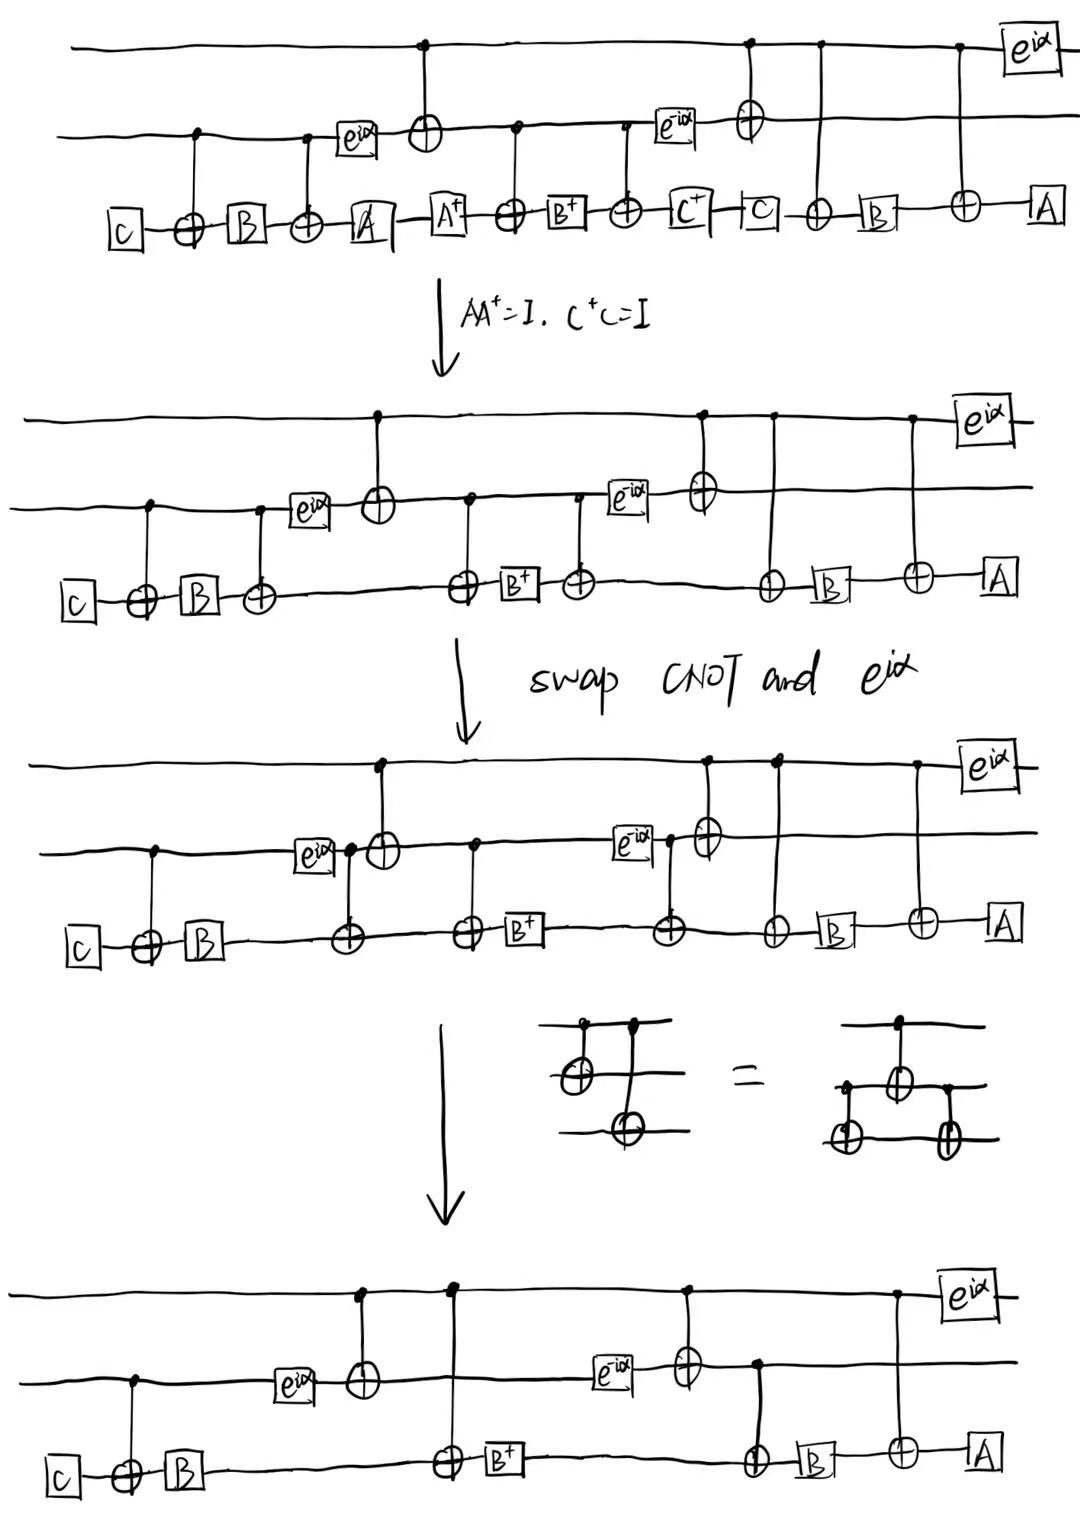
\includegraphics[width=0.8\textwidth]{figures/4-22.jpg}
    \caption{}
    \label{}
\end{figure}

\subsection*{Exercise 4.23}
We should just find proper gates for this decomposition:
\begin{figure}[htbp]
    \centering
    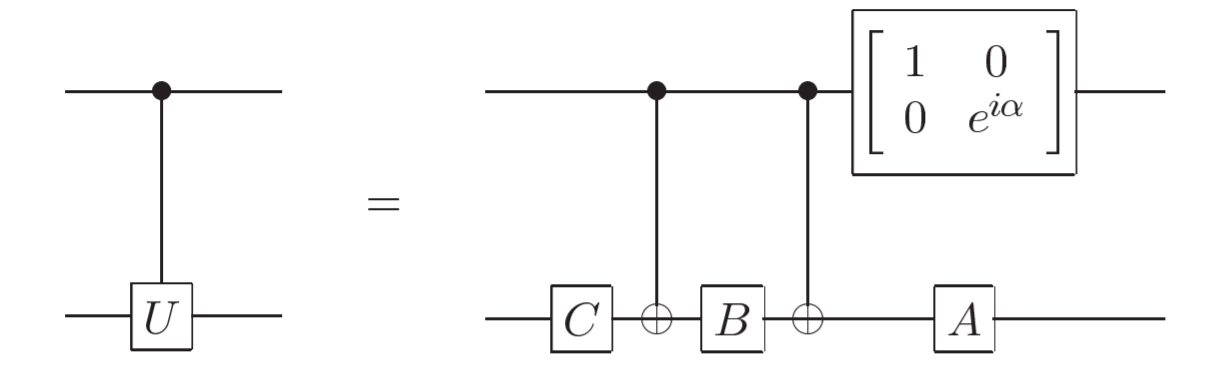
\includegraphics[width=0.8\textwidth]{figures/4-23.jpg}
    \caption{}
    \label{}
\end{figure}

If $U=R_y(\theta)$, then $e^{i\alpha}=\det(U)$ and $\alpha=0$. Therefore, we can just let $\alpha=0, A=I,B=R_y(-\theta/2)$ and $C=R_y(\theta/2)$.

As for $U=R_x(\theta)$, we can similarly rotate the system, and then apply $HZH=X$. Therefore, we can just let $\alpha = 0, A = H, B =R_z(-\theta/2)$ and $C=HR_y(\theta/2)$.

\subsection*{Exercise 4.30}

To achieve $C^n(U)$, we can first achieve it using $C^n(X)$ and other single qubit gates, and then the problem is how to achieve $C^n(X)$ using Tollifo gates and single qubit gates without work qibits.

To do this, we can let $A^2=X$, and apply $O(n^2)$ $C^2(A)$ gates and $C^2(X)$ gates.

\end{document}  